\documentclass[10pt,conference]{IEEEtran}
\usepackage{graphicx}
\usepackage{booktabs}
\usepackage{siunitx}
\usepackage{subcaption}
\usepackage{hyperref}
\usepackage{amsmath}
\usepackage{listings}
\usepackage{xcolor}
\usepackage{float}
\usepackage{tikz}
\usetikzlibrary{arrows.meta,positioning,fit}

% Graphics live in repo plots
\graphicspath{{../results/plots/}}

\title{Mixed-Precision Matrix Multiplication on FPGA: Architecture, Measurement, and Trade-offs}

\author{\IEEEauthorblockN{Ashwin Sabani}
\IEEEauthorblockA{Email: ashwin@example.com}}

\begin{document}
\maketitle

\begin{abstract}
We present a compact, parameterizable mixed-precision GEMM pipeline that targets INT8, FP16, and FP32, implemented in SystemVerilog and instrumented with a hardware-aware results suite. The design exposes precision at the processing element and composes under a controller for matrix multiply with on-chip BRAM. We evaluate accuracy and throughput using the experiment logs included in this repository. On 8\,$\times$\,8 matrices, FP16 tracks FP32 accuracy for well-conditioned inputs while INT8 requires explicit scaling to avoid large bias. We report simulated throughput, error statistics, and range utilization, and discuss how to extend the design toward a RISC-V accelerator or larger systolic arrays.
\end{abstract}

\section{Introduction}
Matrix multiplication dominates modern ML and scientific codes. The choice of numeric format drives the balance among accuracy, bandwidth, area, and power. The community often drops from FP32 to FP16 or INT8 for inference, but the reasons span more than the arithmetic units; storage and memory movement matter as much.

Our goal is a clear mixed-precision GEMM pipeline whose precision can be selected without touching control logic. The design is written in SystemVerilog, uses BRAM-backed matrices, and reports both numerical and hardware-aware metrics. This paper documents the architecture and presents results drawn directly from the CSVs and plots included with this project.

\subsection{Background}
\textbf{RISC-V INT8.} The RISC-V vector and packed-SIMD extensions provide integer dot products that execute multiple INT8 multiplies and accumulations per instruction. INT8 reduces traffic fourfold versus FP32 and increases arithmetic density, which is critical for bandwidth-bound inference. Correct range management and accumulation width are essential to avoid saturation and sign errors \cite{jacob2018quantization}.

\textbf{FP16 on RISC-V.} The Zfh extension introduces IEEE 754 half precision \cite{riscv_zfh,ieee754}. FP16 halves storage versus FP32 and often doubles effective register bandwidth. Many hardware implementations flush subnormals and simplify rounding to keep latency low; this can affect ill-conditioned problems. With values scaled into range, FP16 typically tracks FP32 closely on common workloads.

\textbf{Why mixed precision.} No single format is best across layers, matrices, or devices. A pipeline that can be built for INT8, FP16, or FP32 lets a system choose the format that fits accuracy and energy targets for each stage.

\section{Architecture}
The pipeline composes a processing element (PE) into a controller-driven GEMM with row-major BRAM interfaces. Precision is a parameter that flows through the PE and can be selected at build time.

\textbf{Precision definitions.} The package \texttt{mp\_types.sv} defines the precision enum with \texttt{PREC\_INT8}, \texttt{PREC\_FP16}, and \texttt{PREC\_FP32}, and allows an override via a preprocessor define. INT8 data width is 8\,bits with a 32\,bit accumulator; FP16 and FP32 follow IEEE 754.

\textbf{Processing element.} The PE computes \(\text{acc} \leftarrow \text{acc} + a\cdot b\): INT8 uses a signed 8\,bit multiply widened to 16\,bit, accumulated into 32\,bit; FP16 and FP32 paths wrap multiply and add units and form a two-stage pipeline.

\textbf{Controller.} A state machine streams A and B from BRAM, performs \(K\) MACs per output element, and writes back C. Indices are row-major, and a debug port can read back C.

\textbf{Array shell.} A minimal systolic shell is provided for scaling to \(N\times N\) tiles, though the measurements here use the single-PE controller for clarity.

\begin{figure}[H]
  \centering
  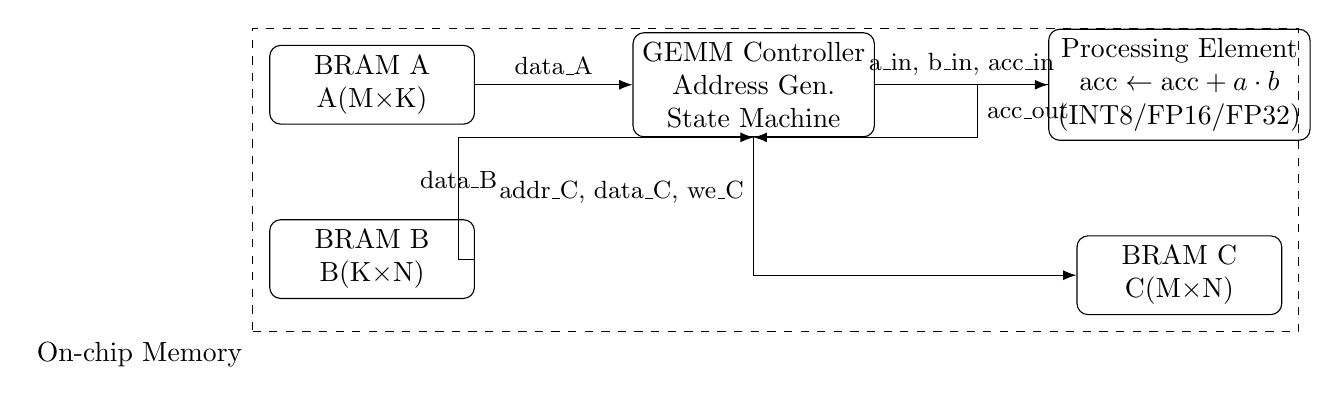
\begin{tikzpicture}[
      block/.style={draw, rounded corners, align=center, minimum width=2.6cm, minimum height=1.0cm},
      smallblock/.style={draw, rounded corners, align=center, minimum width=2.0cm, minimum height=0.9cm},
      >=LaTeX
    ]
    % Nodes
    \node[block] (bramA) {BRAM A\\A(M$\times$K)};
    \node[block, right=2.0cm of bramA] (ctrl) {GEMM Controller\\Address Gen. \\ State Machine};
    \node[smallblock, right=2.2cm of ctrl] (pe) {Processing Element\\$\text{acc} \leftarrow \text{acc}+a\cdot b$\\(INT8/FP16/FP32)};
    \node[block, below=1.2cm of bramA] (bramB) {BRAM B\\B(K$\times$N)};
    \node[block, below=1.2cm of pe] (bramC) {BRAM C\\C(M$\times$N)};

    % Arrows for reads
    \draw[->] (bramA) -- node[midway, above]{\small data\_A} (ctrl);
    \draw[->] (bramB) -- ++(1.1,0) |- node[pos=0.25, above]{\small data\_B} (ctrl.south);
    % From controller to PE
    \draw[->] (ctrl) -- node[midway, above]{\small a\_in, b\_in, acc\_in} (pe);
    % From PE back to controller (acc update)
    \draw[->] (pe.west) -- ++(-0.9,0) |- node[pos=0.25, right]{\small acc\_out} (ctrl.south);
    % Write C
    \draw[->] (ctrl.south) |- node[pos=0.2, left]{\small addr\_C, data\_C, we\_C} (bramC);

    % Optional dashed fit around data memories
    \node[draw, dashed, fit=(bramA)(bramB)(bramC), inner sep=6pt, label={[align=center]south west:On-chip Memory}] {};
  \end{tikzpicture}
  \caption{Block diagram of the mixed-precision GEMM pipeline showing BRAM-backed operands, controller, and the precision-parameterized processing element.}
  \label{fig:block}
\end{figure}

\begin{figure}[H]
  \centering
  \includegraphics[width=0.9\linewidth]{10_comprehensive_dashboard.png}
  \caption{Dashboard plot from this repo summarizing error and performance metrics for a representative run.}
  \label{fig:dashboard}
\end{figure}

\section{Methods}
\textbf{Data.} Inputs are synthetic 8\,$\times$\,8 matrices with recorded requested and measured condition numbers for A and B. Values are bounded to small ranges to keep FP16 within dynamic range without special handling.

\textbf{Simulation.} Cycle-accurate SystemVerilog simulation. The same GEMM program is run under INT8, FP16, and FP32, and results are written to CSV along with derived hardware-aware metrics.

\textbf{Metrics.} We use the columns documented in the repository's metrics file \cite{this_repo_metrics}, including throughput (ops/s, GOPS), accuracy (MAE, RMSE, percentiles), floating-point ULP error, error-shape indicators (RMSE/MAE, p99/p50), range utilization for INT8, and sign-error counts.

\section{Results}
We summarize observations from the CSVs in this project for 8\,$\times$\,8 GEMM.

\subsection{Throughput}
All three precisions report simulated throughput in a similar band for these small matrices. Median operations per second from the CSV with hardware metrics are shown in Table~\ref{tab:medians}. These should be interpreted as relative simulation values, not device-level claims.

\begin{table}[H]
  \centering
  \sisetup{round-mode=places,round-precision=3}
  \caption{Medians across runs from \texttt{results/comprehensive\_results\_with\_hw\_metrics.csv}.}
  \label{tab:medians}
  \begin{tabular}{l S[table-format=3.3] S[table-format=7.3] S[table-format=7.3]}
    \toprule
    Precision & {Median ops/s} & {Median RMSE} & {Median MAE} \\
    \midrule
    INT8 & 140.590 & 2563785.896 & 2172450.727 \\
    FP16 & 137.534 & 2.840 & 2.091 \\
    FP32 & 143.974 & 3.106 & 2.372 \\
    \bottomrule
  \end{tabular}
\end{table}

\subsection{Accuracy}
FP16 closely tracks FP32 on these inputs, with single-digit MAE/RMSE in both modes. Representative FP16 rows show \texttt{ulp\_error\_mean} near 1 and \texttt{ulp\_error\_max} below 2, consistent with correct rounding for well-conditioned cases. INT8, run without per-tile scaling, shows large bias and error due to full-range utilization and saturation, as seen in the CSV columns \texttt{int8\_range\_utilization\_pct} (often 100) and \texttt{bias\_fraction} (often near 1).

\begin{figure}[H]
  \centering
  \includegraphics[width=0.9\linewidth]{05_error_distribution_shape.png}
  \caption{Error distribution shape: RMSE/MAE and interquartile spread highlight outliers.}
  \label{fig:errshape}
\end{figure}

\subsection{Range Utilization and Sign Errors}
For INT8, range utilization is high without scaling, increasing the chance of saturation and sign errors. The INT8 trail shows high \texttt{sign\_error\_count} and \texttt{sign\_error\_pct} in some runs, signaling catastrophic direction flips that require mitigation.

\begin{figure}[H]
  \centering
  \includegraphics[width=0.9\linewidth]{04_int8_range_util.png}
  \caption{INT8 range utilization in representative runs. Values near 100\% indicate little headroom.}
  \label{fig:int8range}
\end{figure}

\subsection{Pareto View}
The Pareto plot mixes normalized throughput with accuracy. FP16 dominates many well-conditioned cases; INT8 improves once accuracy constraints are relaxed or proper scaling is introduced.

\begin{figure}[H]
  \centering
  \includegraphics[width=0.9\linewidth]{01_pareto_plot.png}
  \caption{Pareto trade-off between simulated throughput and accuracy.}
\label{fig:pareto}
\end{figure}

\begin{figure}[H]
  \centering
  \includegraphics[width=0.9\linewidth]{07_performance_scaling.png}
  \caption{Simulated performance scaling across test conditions in this repo.}
  \label{fig:perfscale}
\end{figure}

\section{Discussion}
\textbf{Precision and accumulation.} INT8 is compelling for bandwidth and area, but requires a scaling policy and, for larger \(K\), either block floating-point or a wider accumulator. FP16 can accumulate in FP16 for speed or in FP32 for stability.

\textbf{Controller and memory.} With a single PE, BRAM bandwidth is sufficient. Scaling to an array demands careful tiling and reuse to keep the array fed. The systolic shell can amortize A and B reads and increase arithmetic intensity.

\textbf{Mapping to RISC-V.} The INT8 PE aligns with vector dot-product instructions in RISC-V, and FP16 maps to Zfh units. The metrics used here—throughput, range utilization, sign errors—carry over to bring-up on a RISC-V SoC.

\section{Limitations}
Simulation time dominates the throughput metrics, so we use them for relative comparison only. Matrices are small (8\,$\times$\,8), which understates pipeline fill/drain effects present in larger arrays. INT8 results are intentionally unscaled to expose raw behavior.

\section{Future Work}
Add per-tile scaling and block floating-point for INT8; accumulate FP16 into FP32 for ill-conditioned inputs; scale the systolic array and add a memory model to estimate device-level throughput; and integrate a RISC-V host to stream tiles on hardware.

\section{Conclusion}
A small, modular mixed-precision GEMM pipeline makes precision trade-offs explicit. FP16 delivers accuracy close to FP32 on these inputs. INT8 achieves compact data movement but requires scaling to avoid bias. The architecture here is a practical base for a RISC-V accelerator or FPGA prototype.

\bibliographystyle{IEEEtran}
\bibliography{references}

\end{document}
